
The task of an LLVM backend is to create machine instructions from the LLVM IR. This process is called instruction selection or lowering. Motivated by the idea to automate this task as much as possible, the LLVM developers invented the TableGen language to capture all the details of a target description. We first look at this language before diving into the instruction selection algorithms.\par

\hspace*{\fill} \par %插入空行
\textbf{Specifying the target description in the TableGen language}

A machine instruction has a lot of properties: a mnemonic used by the assembler and disassembler, a bit pattern to represent the instruction in memory, input and output operands, and so on. The LLVM developers decided to capture all this information in a single place, the target description. A new language, the TableGen language, was invented for this purpose. The idea was to use a code generator to create various source fragments from the target description, which could then be used in different tools. Target descriptions are stored in files using the .td suffix.\par

In principle, the TableGen language is very simple. All you can do is define records. A record has a unique name and contains a list of values and a list of superclasses. A definition is a record in which all values are defined, while a class is a record that can have undefined values. The main purpose of classes is to have an abstract record that can be used to build other abstract or concrete records. For example, the Register class defines the common properties of a register, and you can define a concrete record for register R0:\par

\begin{lstlisting}[caption={}]
class Register {
	string name;
}

def R0 : Register {
	let name = "R0";
	string altName = "$0";
}
\end{lstlisting}

You use the let keyword to override a value.\par

The TableGen language has a lot of syntactic sugar to make dealing with records easier. A class can have a template argument, for example:\par

\begin{lstlisting}[caption={}]
class Register<string n> {
	string name = n;
}

def R0 : Register<"R0"> {
	string altName = "$0";
}
\end{lstlisting}

The TableGen language is statically typed, and you have to specify the type of each value. Some of the supported types are the following:\par

\begin{itemize}
	\item bit: A single bit
	\item int: A 64-bit integer value
	\item bits<n>: An integral type consisting of n bits
	\item string: A character string
	\item list<t>: A list of elements of type t
	\item dag: A directed acyclic graph (DAG; used by the instruction selection)
\end{itemize}

The name of a class can also be used as a type. For example, list<Register> specifies a list of elements of the Register class.\par

The language allows the inclusion of other files with the include keyword. For  conditional compiling, the preprocessor directives \#define, \#ifdef, and \#ifndef are supported.\par

The TableGen library in LLVM can parse files written in the TableGen language and create an in-memory representation of the records. You can use this library to create your own generator.\par

LLVM comes with its own generator tool called llvm-tblgen and some .td files. The target description of a backend includes the llvm/Target/Target.td file first. This file defines classes such as Register, Target, or Processor. The llvm-tblgen tool knows about these classes and generates C++ code from the defined records.\par

Let's have a look at the MIPS backend as an example. The target description is in the Mips.td file in the llvm/lib/Target/Mips folder. This file includes the Target.td file mentioned first. It also defines target features, for example:\par

\begin{tcolorbox}[colback=white,colframe=black]
def FeatureMips64r2 \\
\hspace*{0.5cm}: SubtargetFeature<"mips64r2", "MipsArchVersion",  \\
\hspace*{4cm}"Mips64r2", "Mips64r2 ISA Support", \\
\hspace*{4cm}[FeatureMips64, FeatureMips32r2]>;
\end{tcolorbox}

Such features are later used to define CPU models, for example:\par

\begin{tcolorbox}[colback=white,colframe=black]
def : Proc<"mips64r2", [FeatureMips64r2]>;
\end{tcolorbox}

Other files that define registers, instructions, scheduling models, and so on are also included.\par

The llvm-tblgen tool can show you the records defined by this target description. If you are in the build directory, then the following command will print the records to the console:\par

\begin{tcolorbox}[colback=white,colframe=black]
\$ bin/llvm-tblgen $\setminus$ \\
\hspace*{0.5cm}-I../llvm-project/llvm/lib/Target/Mips/ $\setminus$ \\
\hspace*{0.5cm}-I../llvm-project/llvm/include $\setminus$ \\
\hspace*{0.5cm}../llvm-project/llvm/lib/Target/Mips/Mips.td
\end{tcolorbox}

Like with Clang, the –I option adds a directory to search when including files. To see the records can be helpful for debugging. The real purpose of the tool is to generate C++ code from the records. For example, with the -gen-subtarget option, the data necessary to parse the –mcpu= and –mtarget= option of llc is emitted to the console:\par

\begin{tcolorbox}[colback=white,colframe=black]
\$ bin/llvm-tblgen $\setminus$ \\
\hspace*{0.5cm}-I../llvm-project/llvm/lib/Target/Mips/ $\setminus$ \\
\hspace*{0.5cm}-I../llvm-project/llvm/include $\setminus$ \\
\hspace*{0.5cm}../llvm-project/llvm/lib/Target/Mips/Mips.td $\setminus$ \\
\hspace*{0.5cm}-gen-subtarget
\end{tcolorbox}

Save the generated code from that command in a file and explore how the feature and the CPU are used in generated code!\par

The encoding of instructions usually follows a handful of patterns. Therefore, the definition of instructions is split into classes defining the bit encoding and the concrete definition of instruction. The encoding for the MIPS instructions is in the file llvm/Target/Mips/MipsInstrFormats.td. Let's have a look at the definition of the ADD\underline{~}FM format:\par

\begin{tcolorbox}[colback=white,colframe=black]
class ADD\underline{~}FM<bits<6> op, bits<6> funct> : StdArch \{ \\
\hspace*{0.5cm}	bits<5> rd; \\
\hspace*{0.5cm}	bits<5> rs; \\
\hspace*{0.5cm}	bits<5> rt; \\
\\
\hspace*{0.5cm}	bits<32> Inst; \\
\\
\hspace*{0.5cm}	let Inst{31-26} = op; \\
\hspace*{0.5cm}	let Inst{25-21} = rs; \\
\hspace*{0.5cm}	let Inst{20-16} = rt; \\
\hspace*{0.5cm}	let Inst{15-11} = rd; \\
\hspace*{0.5cm}	let Inst{10-6} = 0; \\
\hspace*{0.5cm}	let Inst{5-0} = funct; \\
\}
\end{tcolorbox}

In the record body, several new bit fields are defined: rd, rs, and so on. They are used to override portions of the Inst field, which holds the bit pattern for the instruction. The rd, rs, and rt bit fields encode the registers the instruction operates on, and the op and funct parameters denote the opcode and a function number. The StdArch superclass only adds a field stating that this format follows a standard encoding.\par

Most instruction encoding in the MIPS target does not refer to the DAG nodes and do not specify the assembly mnemonic. A separate class is defined for that. One of the instructions in the MIPS architecture is the nor instruction, which computes the bitwise or of the first and second input register, inverts the bits of the result, and assigns the result to the output register. There are several variants of this instruction, and the following LogicNOR class helps with avoiding the same definitions multiple times:\par

\begin{tcolorbox}[colback=white,colframe=black]
class LogicNOR<string opstr, RegisterOperand RO>: \\
\hspace*{0.5cm}InstSE<(outs RO:\$rd), (ins RO:\$rs, RO:\$rt), \\
\hspace*{3cm}!strconcat(opstr, "\t\$rd, \$rs, \$rt"), \\
\hspace*{3cm}[(set RO:\$rd, (not (or RO:\$rs, RO:\$rt)))], \\
\hspace*{3cm}II\underline{~}NOR, FrmR, opstr> \{ \\
\hspace*{0.5cm}let isCommutable = 1; \\
\}
\end{tcolorbox}

Wow, the simple concept of records now looks complicated. Let's dissect that definition. The class derives from the InstSE class, which is always used for instructions with standard encoding. If you follow the superclass hierarchy further, then you see that this class derives from Instruction class, which is the predefined class denoting an instruction of a target. The (outs RO:\$rd) parameter defines the result of the final instruction as a DAG node. The RO part refers to the parameter of the same name of the LogicNOR class and denotes a register operand. The \$rd is the register to use. This is the value that will be put later into the instruction encoding, in the rd field. The second parameter defines the values the instruction will operate on. In summary, this class is for an instruction that operates on three registers. The !strconcat(opstr, "$\setminus$t\$rd, \$rs, \$rt") parameter assembles the textual representation of the instruction. The !strconcat operator is a predefined functionality from TableGen, which concatenates two strings. You can look up all predefined operators in the TableGen programmer's guide at: \url{https://llvm.org/docs/TableGen/ProgRef.html}.\par

It follows a pattern definition, which resembles the textual description of the nor instruction and describes the computation of this instruction. The first element of the pattern is the operation, which is followed by a comma-separated list of operands. The operands refer to the register names in the DAG parameters and also specify an LLVM IR value type. LLVM has a set of predefined operators, such as add and and, which can be used in patterns. The operators are of the SDNode class, and can also beused as parameters. You can look up the predefined operators in the file llvm/Target/TargetSelectionDAG.td.\par

The II\underline{~}NOR parameter specifies the itinerary class used in the scheduling model, and the FrmR parameter is a value defined to identify this instruction format. Finally, the opstr mnemonic is passed to the superclass. The body of this class is quite simple: it just specifies that the nor operation is commutative, which means that the order of the operands can be swapped.\par

Finally, this class is used to define a record for an instruction, as an example, for the nor instruction in 64-bit mode:\par

\begin{tcolorbox}[colback=white,colframe=black]
def NOR64 : LogicNOR<"nor", GPR64Opnd>, ADD\underline{~}FM<0, 0x27>,  \\
\hspace*{6cm}GPR\underline{~}64;
\end{tcolorbox}

This is the final definition, recognizable from the def keyword. It uses the LogicNOR class to define the DAG operands and pattern, and the ADD\underline{~}FM class to specify the binary instruction encoding. The additional GPR\underline{~}64 predicate makes sure that this instruction is only used if 64-bit registers are available.\par

The developers try hard to not repeat definitions multiple times, and one often-used approach is the use of multiclass classes. A multiclass class can define multiple records at once.\par

For example, the floating point unit of a MIPS CPU can perform addition with single- or double-precision floating point values. The definition of both instructions is very similar, therefore a multiclass class is defined to create two instructions at once:\par

\begin{tcolorbox}[colback=white,colframe=black]
multiclass ADDS\underline{~}M<…> \{ \\
\hspace*{1cm}def \underline{~}D32 : ADDS\underline{~}FT<…>, FGR\underline{~}32; \\
\hspace*{1cm}def \underline{~}D64 : ADDS\underline{~}FT<…>, FGR\underline{~}64; \\
\}
\end{tcolorbox}

The ADDS\underline{~}FT class defines the instruction format, similar to the LogicNOR class. The FGR\underline{~}32 and FGR\underline{~}64 predicates are used to decide at compile time which instruction can be used. The important part is the definition of \underline{~}D32 and \underline{~}D64 records. These are the templates for the records. The instruction records are then defined with the defm keyword:\par

\begin{tcolorbox}[colback=white,colframe=black]
defm FADD : ADDS\underline{~}M<…>;
\end{tcolorbox}

This defines the two records from the multiclass at once and assigns the names FADD\underline{~}D32 and FADD\underline{~}D64 to them. This is a very powerful way to avoid code repetition, and it is often used in the target descriptions, but combined with the other TableGen features it can lead to very cryptic definitions.\par

With the knowledge of how the target description is organized, we can now explore the instruction selection in the next section.\par

\hspace*{\fill} \par %插入空行
\textbf{Instruction selection with the selection DAG}

The standard way LLVM converts the IR to machine instructions is via a DAG. Using pattern matching with the patterns provided in the target description and using custom code, the IR instructions are transformed into machine instructions. This approach is not as straightforward as it sounds: the IR is mostly target-independent and can contain data types that are not supported on the target. For example, the i1 type representing a single bit is not a valid type on most targets.\par

The selectionDAG consists of nodes of SDNode type, defined in the file llvm/CodeGen/SelectionDAGNodes.h. The operation the node represents is called OpCode, and the target-independent codes are defined in the file llvm/CodeGen/ISDOpcodes.h. Besides the operation, the node stores the operands and the value it produces.\par

The values and operands of a node form a data flow dependency. A control flow dependency is represented by chain edges, which have the special type MVT::Other. This makes it possible to keep the order of instructions with side effects, for example, a load instruction.\par

Instruction selection using the selection DAG is performed with the following steps:\par

\begin{enumerate}
\item The DAG is constructed
\item The DAG is optimized.
\item The types in the DAG are legalized
\item The DAG is optimized.
\item The operations in the DAG are legalized.
\item The instructions are selected.
\item The instructions are ordered.
\end{enumerate}

Let's examine how we can follow the changes each of the steps makes to the selection DAG.\par

\hspace*{\fill} \par %插入空行
\textbf{How to follow the instruction selection process}

You can see the work of the instruction selection in two different ways. If you pass the –debug-only=isel option to the llc tool, then the result of each step is printed in textual format. This is a great help if you need to investigate why a machine instruction was selected. For example, run the following command to see the output for the sum.ll file from the Understanding the LLVM target backend structure section:\par

\begin{tcolorbox}[colback=white,colframe=black]
\$ llc -mtriple=mips-linux-gnu -debug-only=isel < sum.ll
\end{tcolorbox}

This prints a lot of information. At the top of the output, you see the description of the initial created DAG for the input:\par

\begin{tcolorbox}[colback=white,colframe=black]
Initial selection DAG: \%bb.0 'sum:' \\
SelectionDAG has 12 nodes: \\
\hspace*{0.5cm}t0: ch = EntryToken \\
\hspace*{2.5cm}t2: i32,ch = CopyFromReg t0, Register:i32 \%0 \\
\hspace*{2cm}t5: i16 = truncate t2 \\
\hspace*{2.5cm}t4: i32,ch = CopyFromReg t0, Register:i32 \%1 \\
\hspace*{2cm}t6: i16 = truncate t4 \\
\hspace*{1.5cm}t7: i16 = add t5, t6 \\
\hspace*{1cm}t8: i32 = any\underline{~}extend t7 \\
\hspace*{0.5cm}t10: ch,glue = CopyToReg t0, Register:i32 \$v0, t8 \\
\hspace*{0.5cm}t11: ch = MipsISD::Ret t10, Register:i32 \$v0, t10:1 
\end{tcolorbox}

Like in the MIR output from the last section, you see here CopyFromReg instructions, which transfer the content of registers used by the ABI to virtual nodes. The truncate nodes are required because the example uses 16-bit values, but the MIPS architectures have only native support for 32-bit values. The add operation is performed on 16-bit virtual registers, and the result is extended and returned to the caller. Such a section is  printed for each of the steps mentioned above.\par

LLVM can also generate a visualization of the selection DAG with the help of the Graphviz software. If you pass the –view-dag-combine1-dags option to the llc tool, then a window opens showing the constructed DAG. For example, run llc with the small file from the preceding:\par

\begin{tcolorbox}[colback=white,colframe=black]
\$ llc -mtriple=mips-linux-gnu –view-dag-combine1-dags sum.ll
\end{tcolorbox}

Running on a Windows PC, you then see the DAG:\par

\hspace*{\fill} \par %插入空行
\begin{center}
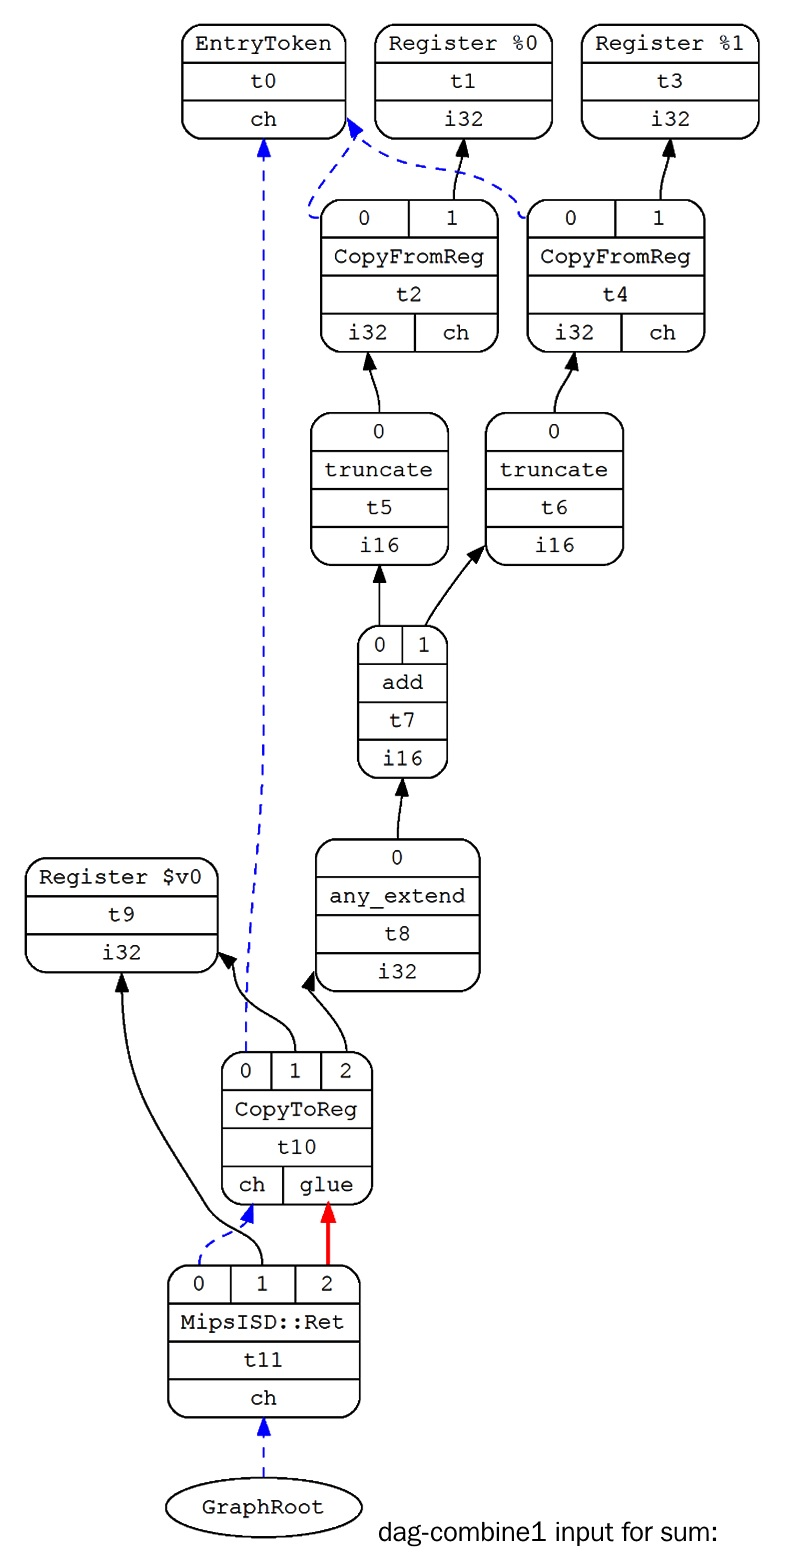
\includegraphics[width=0.55\textwidth]{content/3/chapter9/images/1.jpg}\\
Figure 9.1 – Constructed selection DAG for the sum.ll file
\end{center}

Be sure to compare that the textual representation and this graph contain the same information. The EntryToken is the start of the DAG, and the GraphRoot is the final node. The chain for the control flow is marked with the blue dashed arrows. The black arrows denote the data flow. The red arrows glue nodes together, preventing reordering them. The graph can get really big even for moderately sized functions. It does not contain more or other information than the textual output with the –debug-only=isel option, only the presentation is more comfortable. You can also generate the graph at other points in time, for example:\par

\begin{itemize}
\item Add the \verb|--|view-legalize-types-dags option to see the DAG before 
type legalization.
\item Add the –view-isel-dags option to see the selection instructions
\end{itemize}

You can see all available options to view the DAG using the \verb|--|help-hidden option. Because the DAG can get large and confusing, you can limit the rendering to one basic block using the -filter-view-dags option.\par

\hspace*{\fill} \par %插入空行
\textbf{Examining the instruction selection}

Knowing how to visualize the DAG, we can now dive into the details. The selection DAG is constructed from the IR. For each function in the IR, an instance of the SelectionDAG class is populated by the SelectionDAGBuilder class. There are no special optimizations done at this step. Nevertheless, a target needs to provide some functions to lower calls, argument handling, return jumps, and so on. To do so, the target has to implement the TargetLowering interface. Inside the folder of a target, the source is usually in the XXXISelLowering.h and XXXISelLowering.cpp files. The implementation of the TargetLowering interface provides all the information needed for the instruction process, for example, which data types and which operations are supported on the target.\par

The optimization step is run several times. The optimizer performs simple optimization, for example identifying rotates on targets that support these operations. The rationale here is that a cleaned-up DAG is produced, which simplifies the other steps.\par

During the type legalization step, types that are not supported on the target are replaced with supported ones. For example, if a target natively supports only 32-bit-wide integers, then smaller values must be converted to 32-bit through sign or zero extension. This is called promoting. If a 64-bit value can't be handled by this target, then the value must be split into a pair of 32-bit values. This is called expanding. Vector types are treated similarly. A vector type can be extended with additional elements, or it can be broken up into several values. For example, a vector with four values could be split into two vectors with two values each. If the splitting process ends with a single value, then no suitable vector could be found and scalar types are used instead. This is called scalarizing. The information about the supported types is configured in the target-specific implementation of the TargetLowering interface. After type legalization, the selection DAG has this textual representation for the sum.ll file:\par

\begin{tcolorbox}[colback=white,colframe=black]
Optimized type-legalized selection DAG: \%bb.0 'sum:' \\
SelectionDAG has 9 nodes: \\
\hspace*{0.5cm}t0: ch = EntryToken \\
\hspace*{1.5cm}t2: i32,ch = CopyFromReg t0, Register:i32 \%0 \\
\hspace*{1.5cm}t4: i32,ch = CopyFromReg t0, Register:i32 \%1 \\
\hspace*{1cm}t12: i32 = add t2, t4 \\
\hspace*{0.5cm}t10: ch,glue = CopyToReg t0, Register:i32 \$v0, t12 \\
\hspace*{0.5cm}t11: ch = MipsISD::Ret t10, Register:i32 \$v0, t10:1
\end{tcolorbox}

If you compare this with the initial constructed DAG, then here only 32-bit registers are used. The 16-bit values were promoted, because only 32-bit values are supported natively.\par

Operation legalization is similar to type legalization. This step is necessary because not all operations may be supported by a target, or even if a type is natively supported on a target, it may not valid for all operations. For example, not all targets have a native instruction for population count. In such cases, the operation is replaced by a sequence of operations to implement the functionality. If the type does not fit for the operation, then promoting the type to a larger one could be done. It is also possible for a backend author to provide custom code. If the legalization action is set to Custom, then the LowerOperation() method in the TargetLowering class is called for these operations. The method must create a legal version of the operation then. In the sum.ll example, the add operation is already legal, because addition of two 23-bit registers is supported on the platform, and nothing changed.\par

After types and operations are legalized, the instruction selection happens. A large part of the selection is automated. Remember from the previous section that you provided a pattern in the description of an instruction. From these descriptions, a pattern matcher is generated by the llvm-tblgen tool. Basically, the pattern matcher tries to find a pattern that matches the current DAG node. The instruction associated with the pattern will then be selected. The pattern matcher is implemented as a bytecode interpreter. The available codes for the interpreter are defined in the llvm/CodeGen/SelectionDAGISel.h header file. The XXXISelDAGToDAG class implements the instruction selection for a target. The Select() method is called for each DAG node. The default is to call the generated matcher, but you can also add code for cases not handled by it.\par

It is noteworthy that there is no one-to-one relationship between a selection DAG node and the selected instructions. A DAG node can expand into several instructions, and several DAG nodes can collapse into a single instruction. An example of the former is synthesizing immediate values. Especially on RISC architectures, the bit length of immediate values is restricted. A 32-bit target may only support an embedded immediate value of 16-bit length. To perform an operation that requires a 32-bit constant value, you usually split it into two 16-bit values and then generate two or more instructions that use the 16-bit values instead. Among others, you find patterns for this in the MIPS target. Bit-field instructions are a common example for the latter case: combinations of and, or, and shift DAG nodes can often be matched to special bit-field instructions, resulting in just one instruction for two or more DAG nodes.\par

Usually, you specify a pattern in the target description to combine two or more DAG nodes. For more complex cases, which are not easily handled with a pattern, you can mark the operation of the top node to require special DAG combine treatment. For these nodes, the PerformDAGCombine() method in the XXXISelLowering class is called. You can then check arbitrary complex patterns, and if you find your match, then you can return the operation representing the combined DAG nodes. This method is called before the generated matcher is run for the DAG node.\par

You can follow the instruction selection process in the printed output for the sum.ll file. For the add operation, you find there the following lines:\par

\begin{tcolorbox}[colback=white,colframe=black]
ISEL: Starting selection on root node: t12: i32 = add t2, t4 \\
ISEL: Starting pattern match \\
\hspace*{0.5cm}Initial Opcode index to 27835 \\
\hspace*{0.5cm}… \\
\hspace*{0.5cm}Morphed node: t12: i32 = ADDu t2, t4 \\
ISEL: Match complete!
\end{tcolorbox}

The index numbers point into the array of the generated matcher. The start is at index 27835 (an arbitrary value that can change from release to release), and after some steps, the ADDu instruction is selected.\par

\begin{tcolorbox}[colback=blue!5!white,colframe=blue!75!black, title=Following the pattern matching]
If you encounter a problem with a pattern, then you can also retrace the matching by reading the generated bytecode. You find the source in the lib/Target/XXX/XXXGenDAGIsel.inc file in the build directory. You open the file in a text editor and search for the index in the preceding output. Each line is prefixed with the index number, so you can easily find the right place in the array. The used predicates are also printed as comments, so they can help you to understand why a certain pattern was not selected.
\end{tcolorbox}

\hspace*{\fill} \par %插入空行
\textbf{Turning the DAG into instruction sequences}

After instruction selection, the code is still a graph. This data structure needs to be flattened, which means that the instructions must be sequentially ordered. The graph contains data and control flow dependencies, but there are always several possibilities to order the instructions in such a way that these dependencies are fulfilled. What we want is an order that best utilizes the hardware. Modern hardware can issue several instructions in parallel, but restrictions always apply. A simple example of such a restriction is one instruction requiring the result of another instruction. In such a case, the hardware may not be able to issue both instructions and instead executes the instructions in sequence.\par

You can add a scheduling model to the target description, which describes the available units and their properties. For example, if a CPU has two integer arithmetic units, then this information is captured in the model. For each instruction, it is necessary to know which part of the model is used. There are different ways to do this. The newer, recommended approach is to define a scheduling model using the so-called machineinstruction scheduler. To do so, you need to define a SchedMachineModel record for each subtarget in the target description. Basically, the model consists of definitions for the input and output operands of instructions and processor resources. Both definitions are then associated together with latency values. You can look up the predefined types for this model in the llvm/Target/TargetSched.td file. Look at the Lanai target for a very simple model and in the SystemZ target for a complex scheduling model.\par

There is also an older model based on so-called itineraries. With this model, you define processor units as FuncUnit records. A step using such a unit is defined as an InstrStage record. Each instruction is associated with an itinerary class. For each itinerary class, the used processor pipeline composed of InstrStage records is defined, together with the number of processor cycles required for execution. You can find the predefined types for the itinerary model in the llvm/Target/TargetItinerary.td file.\par

Some targets use both models. One reason is due to development history. The itinerarybased model was the first one added to LLVM, and targets began using this model. When the new machine-instruction scheduler was added more than 5 years later, nobody cared enough to migrate the already existing models. Another reason is that with the itinerary model, you can not only model an instruction that uses multiple processor units, but you can also specify during which cycles the units are used. However, this detail level is rarely needed, and if it is needed, then you can refer to the machine-instruction scheduler model to the defined itineraries, basically pulling this information into the new model too.\par

If present, the scheduling model is used to order the instructions in an optimal way. After this step, the DAG is not needed anymore and is destroyed.\par

Performing instruction selection with the selection DAG produces almost optimal results, but it comes at a cost in terms of runtime and memory usage. Therefore, alternative approaches were developed, which we examine next. In the next section, we look at the fast instruction selection approach.\par

\hspace*{\fill} \par %插入空行
\textbf{Fast instruction selection – FastISel}

Using the selection DAG for instruction selection costs compile time. If you are developing an application, then the runtime of the compiler matters. You also do not care about the generated code so much, because it is more important that complete debug information is emitted. Because of these reasons, the LLVM developers decided to implement a special instruction selector that has a fast runtime but produces less optimal code, and which is used only for –O0 optimization level. This component is called fast instruction selection, or FastIsel for short.\par

The implementation is in the XXXFastISel classes. Not every target supports this instruction selection method, in which case the selection DAG approach is used for –O0, too. The implementation is straightforward: a target-specific class is derived from a FastISel class and has to implement a couple of methods. The TableGen tool generates most of the required code from the target description. Nevertheless, there is some effort needed to implement this instruction selector. One of the root causes is that you need to get the calling convention right, which is usually complex.\par

The MIPS target features an implementation of fast instruction selection. You can enable use of fast instruction selection by passing the –fast-isel option to llc tool. Using the sum.ll example file from first section, an invocation looks like this:\par

\begin{tcolorbox}[colback=white,colframe=black]
\$ llc -mtriple=mips-linux-gnu -fast-isel –O0 sum.ll
\end{tcolorbox}

Fast instruction selection runs very quickly, but it is a completely different code path. Some LLVM developers decided to look for a solution that runs quickly but can also produce good code, with the goal to replace both the selection dag and the fast instruction selector in the future. We look at this approach in the next section.\par

\hspace*{\fill} \par %插入空行
\textbf{The new global instruction selection – GlobalISel}

Using the selection DAG, we can generate pretty good machine code. The drawback is that it is a very complex piece of software. This means that it is hard to develop, test, and maintain. The FastISel instruction selection works quickly and is less complex, but does not produce good code. Both approaches do not share much code, except for the code generated by TableGen.\par

Can we have the best of both worlds? One instruction selection algorithm, which is fast, easy to implement, and which produces good code? That is the motivation for adding another instruction selection algorithm, the global instruction selection, to the LLVM framework. The short-term goal is to replace FastISel first, and in the long term the selection DAG, too.\par

The approach taken by global instruction selection is to build on the existing infrastructure. The whole task is broken down into a sequence of machine function passes. Another major design decision is to not introduce another intermediate representation but instead use the existing MachineInstr class. However, new generic opcodes are added.\par

The current sequence of steps is as follows:\par

\begin{enumerate}
\item The IRTranslator pass builds the initial machine instructions using the generic opcodes.

\item The Legalizer pass legalizes types and operations in one step. This is different from the selection DAG, which uses two different steps for it. Real CPU architectures are sometimes weird, and it is possible that a certain data type is only supported with one instruction. This case is not handled well by the selection DAG, but it's easy to handle this in the combined step in the global instruction selection.

\item The generated machine instructions still operate on virtual registers. In the RegBankSelect pass, a register bank is selected. A register bank represents a type of registers on the CPU, for example, general-purpose registers. This is more coarsegrained than the register definitions in the target description. The important point is that it associates type information with the instruction. The type information is based on the types available in the target, so this is already lower than the generic type in LLVM IR.

\item At this point, the types and operations are known to be legal for the target, and type information is associated with each instruction. The following InstructionSelect pass can then easily replace the generic instructions with the machine ones.
\end{enumerate}

After the global instruction selection, the usual backend passes such as instruction scheduling, register allocation, and basic block placement are run.\par

Global instruction selection is compiled into LLVM, but it is not enabled by default. If you want to use it, you need to give the –global-isel option to llc or –mllvm global-isel to clang. You can control what happens if an IR construct cannot be handled by global instruction selection. When you give the -global-isel-abort=0 option to llc, then the selection DAG is used as fallback. With =1, the application is terminated. To prevent this, you can give the -global-isel-abort=0 option to llc. And with =2, the selection DAG is used as fallback, and a diagnostic message is printed to inform you about the problem.\par

To add global instruction selection to a target, you only need to override the corresponding functions in the TargetPassConfig class of your target. This class is instantiated by the XXXTargetMachine class, and the implementation is usually found in the same file. For example, you override the addIRTranslator() method to add the IRTranslator pass to the machine passes of your target.\par

The development happens mainly on the AArch64 target, which currently has the best support for global instruction selection. Many other targets, including x86 and Power, have also added support for global instruction selection. One challenge here is that not that much code is generated from the table description, so there is still an amount of manual coding you have to do. Another challenge is that big-endian targets are currently not supported, so pure big-endian targets such as SystemZ cannot use global instruction selection as of today. Both will certainly improve over time.\par

The Mips target features an implementation of global instruction selection, with the mentioned limitation that it can only be used for little-endian targets. You can enable use of global instruction selection by passing the –global-isel option to the llc tool. Using the sum.ll example file from first section, an invocation looks like this:\par

\begin{tcolorbox}[colback=white,colframe=black]
\$ llc -mtriple=mipsel-linux-gnu -global-isel sum.ll
\end{tcolorbox}

Please note that the target mipsel-linux-gnu is the little-endian target. Using the big-endian mips-linux-gnu target results in an error message.\par

The global instruction selector works much quicker than the selection DAG, and already produces higher code quality than fast instruction selection.\par








